\documentclass[11pt,a4paper]{ctexart}
\usepackage[teacher]{ipara}
\usepackage{mathtools}
\usepackage{longtable}
\raggedbottom

\pagestyle{fancy}
\fancyhf{}
\lhead{\small 高中数学试卷详细解析讲义}
\rhead{\small 教师版：考点分析、方法比较与易错诊断}
\cfoot{\small 第 \thepage\ 页\quad 共 \zpageref{LastPage} 页}
\renewcommand{\headrulewidth}{0.4pt}

\newcommand{\R}{\mathbb{R}}
\newcommand{\dd}{\mathrm{d}}
\newcommand{\ans}[1]{\(\boxed{#1}\)}
\newcommand{\vct}[1]{\overrightarrow{#1}}

\begin{document}

\begin{center}
  {\zihao{2}\bfseries 试卷详细解析讲义}\\[2mm]
  {\Large \bfseries 从答案核对到方法归纳}\\[2mm]
  {\large 适用：高一综合复习 / 试卷讲评课 / 专题补弱课}\\[2mm]
  \rule{0.86\linewidth}{0.5pt}
\end{center}

\begin{teachbox}{使用说明}
本讲义按“先稳定数学答案，再提炼教学价值”的顺序编排。每题给出考点、读题切入口、标准解答和方法点评；立体几何题尽量采用纯几何、截面、折叠不变量、中位线、垂直判定等方法处理，避免一上来建立空间坐标系。
\end{teachbox}

\section{答案速览}

\begin{center}
\small
\begin{tabularx}{0.96\linewidth}{c c c c c c c c c}
\toprule
题号 & 1 & 2 & 3 & 4 & 5 & 6 & 7 & 8\\
\midrule
答案 & C & A & C & D & B & D & B & C\\
\bottomrule
\end{tabularx}
\end{center}

\begin{center}
\small
\begin{tabularx}{0.96\linewidth}{c c c c c c c}
\toprule
题号 & 9 & 10 & 11 & 12 & 13 & 14\\
\midrule
答案 & BD & ACD & ACD & 390 & \(-\dfrac35\) & \(2\sqrt6,\ \dfrac{297\pi}{4}\)\\
\bottomrule
\end{tabularx}
\end{center}

\begin{center}
\small
\begin{tabularx}{0.96\linewidth}{c X}
\toprule
题号 & 解答题结论\\
\midrule
15 & (1) \(m=-\dfrac12\)；(2) \(m>0\)。\\
16 & (1) 由中位线构造平行四边形证明；(2) 线面角为 \(\dfrac{\pi}{4}\)。\\
17 & (1) \(A=\dfrac{\pi}{3}\)；(2) 周长为 \(5+\sqrt7\) 或 \(7+\sqrt{13}\)。\\
18 & (1) 最小值 \(\sqrt{13}\)；(2) 用 \(BD\perp\) 对角面证明；(3) \(\cos\theta\in\left[\dfrac35,\dfrac{\sqrt2}{2}\right]\)。\\
19 & (1) 模的取值范围 \([1,3]\)；(2) 条件不足，不能唯一确定；(3) 不存在点 \(Q\)。\\
\bottomrule
\end{tabularx}
\end{center}

\newpage

\section{选择题详细解析}

\subsection*{第 1 题：复数模的直接计算}
若复数 \(z=i(1-4i)\)，则 \(|z+2i|=\) (\quad) \\
A. 3 \qquad B. 4 \qquad C. 5 \qquad D. 6

\teachblock{考点}{
复数乘法、复数模。此题属于基础送分题，关键是先把 \(z\) 化成代数形式。
}

\teachblock{解答}{
\[
z=i(1-4i)=i-4i^2=4+i.
\]
所以
\[
z+2i=4+3i,\qquad |z+2i|=\sqrt{4^2+3^2}=5.
\]
故选 \ans{C}。
}

\teachblock{方法点评}{
复数题第一步不要急着求模，先化为 \(a+bi\)，再判断实部、虚部、模、象限。卷面上应写清 \(i^2=-1\)，避免符号错导致全题失分。
}

\subsection*{第 2 题：三点共线}
若 \(A(1,-k), B(3,4), C(7,5)\)，且 \(A, B, C\) 三点共线，则 \(k\) 的值为 (\quad) \\
A. \(-\frac{7}{2}\) \qquad B. \(\frac{7}{2}\) \qquad C. -3 \qquad D. 3

\teachblock{考点}{
斜率相等与三点共线。该题训练“坐标条件转化为斜率条件”。
}

\teachblock{解答}{
由 \(B(3,4),C(7,5)\)，得
\[
k_{BC}=\frac{5-4}{7-3}=\frac14.
\]
又
\[
k_{AB}=\frac{4-(-k)}{3-1}=\frac{4+k}{2}.
\]
三点共线，故
\[
\frac{4+k}{2}=\frac14,\qquad k=-\frac72.
\]
故选 \ans{A}。
}

\teachblock{方法点评}{
除了斜率法，本题也可以用“向量共线法”：
\[
\overrightarrow{AB}=(2,4+k),\qquad \overrightarrow{BC}=(4,1).
\]
三点共线等价于 \(\overrightarrow{AB}\parallel \overrightarrow{BC}\)。所以
\[
\frac{2}{4}=\frac{4+k}{1},
\]
解得 \(k=-\frac72\)。这个方法能自然过渡到后面的向量题。

（若用斜率法担心竖直线特例，可先观察 \(x_A,x_B,x_C\) 不相等，不会出现斜率不存在。）
}

\subsection*{第 3 题：锐角三角形的边长范围}
已知锐角三角形边长分别为 2, 3, \(x\)，则 \(x\) 的取值范围是 (\quad) \\
A. \((1,\sqrt{13})\) \qquad B. \((1,5)\) \qquad C. \((\sqrt{5},\sqrt{13})\) \qquad D. 不确定

\teachblock{考点}{
三角形存在性与锐角条件。此题不是只考三角形不等式，还要比较最大边。
}

\teachblock{解答}{
先由三角形不等式得
\[
1<x<5.
\]
锐角三角形要求最大边的平方小于另外两边平方和。

若 \(x\geq 3\)，最大边为 \(x\)，则
\[
x^2<2^2+3^2=13,\qquad x<\sqrt{13}.
\]
若 \(x<3\)，最大边为 \(3\)，则
\[
3^2<2^2+x^2,\qquad x>\sqrt5.
\]
两种情形合并：
\[
\sqrt5<x<\sqrt{13}.
\]
故选 \ans{C}。
}

\teachblock{方法点评}{
本题的易错点是只写 \(1<x<5\)，漏掉锐角条件；或只写 \(x<\sqrt{13}\)，漏掉当 \(3\) 为最大边时的限制。本题核心不是三角形不等式，而是最大边判断。

\textbf{锐角三角形的边长判断口诀：}
先保证能成三角形，再让最大边的平方小于另外两边平方和。最大边不确定时，必须分类。
}

\subsection*{第 4 题：投影向量}
已知单位向量 \(\vec{a}, \vec{b}\) 满足 \(\vec{a}\cdot(\vec{a}+3\vec{b})=0\)，则 \(\vec{a}\) 在 \(\vec{b}\) 上的投影向量为 (\quad) \\
A. \(\vec{b}\) \qquad B. \(-\vec{b}\) \qquad C. \(\frac{1}{3}\vec{b}\) \qquad D. \(-\frac{1}{3}\vec{b}\)

\teachblock{考点}{
单位向量、数量积、投影向量。}

\teachblock{解答}{
因为 \(\vec a,\vec b\) 都是单位向量，且
\[
\vec a\cdot(\vec a+3\vec b)=0,
\]
所以
\[
|\vec a|^2+3\vec a\cdot\vec b=0
\quad\Longrightarrow\quad
1+3\vec a\cdot\vec b=0.
\]
即
\[
\vec a\cdot\vec b=-\frac13.
\]
\(\vec a\) 在 \(\vec b\) 上的投影向量为
\[
\frac{\vec a\cdot\vec b}{|\vec b|^2}\vec b=-\frac13\vec b.
\]
故选 \ans{D}。
}

\teachblock{方法点评}{
注意题目问的是“投影向量”，不是“投影数量”。本题中：
\[
\text{投影数量}=\vec a\cdot \vec b=-\frac13,
\]
但
\[
\text{投影向量}=(\vec a\cdot \vec b)\vec b=-\frac13\vec b.
\]
一定要注意区分“数量”和“向量”的区别。
}

\subsection*{第 5 题：空间位置关系命题}
若 \(m, n, l\) 表示直线，\(\alpha, \beta, \gamma\) 表示平面，则下列命题中，正确命题为 (\quad) \\
A. \(\begin{cases} m \perp l \\ n \perp l \end{cases} \Rightarrow m \parallel n\) \qquad
B. \(\begin{cases} m \perp \alpha \\ n \perp \alpha \end{cases} \Rightarrow m \parallel n\) \\
C. \(\begin{cases} m \perp \alpha \\ m \perp \beta \end{cases} \Rightarrow \alpha \perp \beta\) \qquad
D. \(\begin{cases} \gamma \perp \alpha \\ \gamma \perp \beta \end{cases} \Rightarrow \alpha \parallel \beta\)

\teachblock{考点}{
线线、线面、面面垂直和平行的判定。该题适合训练反例意识。
}

\teachblock{解答}{
\begin{enumerate}[label=\Alph*. , leftmargin=2em, itemsep=0.25em]
  \item 两条直线都垂直于同一直线，不一定平行。例如同一平面内两条不同方向的直线都可以垂直于第三条空间方向的直线。错误。
  \item 两条直线都垂直于同一平面，则它们方向相同或相反，所以平行。正确。
  \item 同一直线同时垂直于两个平面，通常推出两个平面平行，不是垂直。错误。
  \item 同一平面同时垂直于两个平面，不能推出这两个平面平行。例如两个相交平面都可垂直于同一平面。错误。
\end{enumerate}
故选 \ans{B}。
}

\teachblock{方法点评}{
空间命题题的课堂切入口是“先想定理，再找反例”。不能把平面几何中的直观结论直接搬到空间中。
}

\subsection*{第 6 题：四面体中对棱夹角}
在四面体 \(ABCD\) 中，\(E, F\) 分别为棱 \(AC, BD\) 的中点，\(AD=6, BC=4, EF=\sqrt{7}\)，则异面直线 \(AD\) 与 \(BC\) 所成角为 (\quad) \\
A. \(\frac{\pi}{12}\) \qquad B. \(\frac{\pi}{6}\) \qquad C. \(\frac{\pi}{4}\) \qquad D. \(\frac{\pi}{3}\)

\begin{center}
\begin{tikzpicture}[scale=1, >=stealth]
  \coordinate (B) at (0,0);
  \coordinate (C) at (4,0);
  \coordinate (D) at (1.5,1.2);
  \coordinate (A) at (2,3.5);
  
  \draw[dashed, gray, thick] (B) -- (D) -- (C);
  \draw[dashed, gray, thick] (A) -- (D);
  
  \draw[thick] (A) -- (B) -- (C) -- cycle;
  
  \coordinate (E) at ($(A)!0.5!(C)$);
  \coordinate (F) at ($(B)!0.5!(D)$);
  
  \draw[dashed, red, thick] (E) -- (F);
  
  \fill (A) circle (1.5pt) node[above] {\(A\)};
  \fill (B) circle (1.5pt) node[below left] {\(B\)};
  \fill (C) circle (1.5pt) node[below right] {\(C\)};
  \fill (D) circle (1.5pt) node[above right] {\(D\)};
  \fill (E) circle (1.5pt) node[right] {\(E\)};
  \fill (F) circle (1.5pt) node[below right] {\(F\)};
\end{tikzpicture}
\end{center}

\teachblock{考点}{
四面体对棱中点连线公式、异面直线所成角。}

\teachblock{几何切入口}{
设 \(E,F\) 分别为 \(AC,BD\) 的中点，则 \(EF\) 是四面体中连接两组对棱中点的线段。把异面直线 \(AD,BC\) 平移到同一平面中，可得到
\[
EF^2=\frac14\left(AD^2+BC^2-2AD\cdot BC\cos\theta\right),
\]
其中 \(\theta\) 为异面直线 \(AD\) 与 \(BC\) 所成角。
}

\teachblock{解答}{
代入 \(AD=6,BC=4,EF=\sqrt7\)，得
\[
7=\frac14(36+16-48\cos\theta).
\]
于是
\[
28=52-48\cos\theta,\qquad \cos\theta=\frac12.
\]
故
\[
\theta=\frac{\pi}{3}.
\]
故选 \ans{D}。
}

\teachblock{方法点评}{
此题可用向量公式快速算，也可讲成“平移异面直线，构造以 \(AD,BC,2EF\) 为三边的辅助三角形”。课堂上建议把公式来源讲成几何图形，而不是直接套坐标。
}

\subsection*{第 7 题：三角恒等变形与分类}
已知角 \(\alpha, \beta \in (0,\pi)\)，且 \(\sin(\alpha-\beta)+\cos(\alpha+\beta)=0\)，\(\sin\alpha\sin\beta=2\cos\alpha\cos\beta\)，则 \(\tan(\alpha-\beta)=\) (\quad) \\
A. 2 \qquad B. \(\frac{1}{3}\) \qquad C. \(-\frac{1}{3}\) \qquad D. -2

\teachblock{考点}{
和差角公式、正切化简、分类讨论。}

\teachblock{解答}{
由
\[
\sin(\alpha-\beta)+\cos(\alpha+\beta)=0
\]
展开得
\[
\sin\alpha\cos\beta-\cos\alpha\sin\beta+\cos\alpha\cos\beta-\sin\alpha\sin\beta=0,
\]
即
\[
(\sin\alpha+\cos\alpha)(\cos\beta-\sin\beta)=0.
\]
又
\[
\sin\alpha\sin\beta=2\cos\alpha\cos\beta.
\]
由于 \(\alpha,\beta\in(0,\pi)\)，不可能有 \(\cos\alpha\cos\beta=0\)，故
\[
\tan\alpha\tan\beta=2.
\]

若 \(\cos\beta-\sin\beta=0\)，则 \(\tan\beta=1\)，从而 \(\tan\alpha=2\)，
\[
\tan(\alpha-\beta)=\frac{2-1}{1+2\cdot1}=\frac13.
\]
若 \(\sin\alpha+\cos\alpha=0\)，则 \(\tan\alpha=-1\)，从而 \(\tan\beta=-2\)，
\[
\tan(\alpha-\beta)=\frac{-1-(-2)}{1+(-1)(-2)}=\frac13.
\]
故选 \ans{B}。
}

\teachblock{易错提醒}{
不能把 \((\sin\alpha+\cos\alpha)(\cos\beta-\sin\beta)=0\) 只取其中一支；本题两支都要检查，且最终结果相同。
}

\subsection*{第 8 题：单位圆中的线性最值}
已知 \(A, B, C\) 为单位圆 \(O\) (\(O\)为坐标原点) 上不同的三点，且 \(\angle AOB=\frac{2\pi}{3}\)，若 \(\overrightarrow{OC}=\lambda\overrightarrow{OA}+\mu\overrightarrow{OB}\) (\(\lambda, \mu \in \mathbb{R}\))，则当 \(w=(\frac{\sqrt{3}}{2}+1)\lambda+\mu\) 取最大值时，\(\frac{\lambda}{\mu}\) 为 (\quad) \\
A. \(\frac{\sqrt{3}}{2}\) \qquad B. \(\frac{\sqrt{3}+1}{2}\) \qquad C. \(\frac{2\sqrt{3}+10}{11}\) \qquad D. \(\frac{\sqrt{2}}{2}\)

\begin{center}
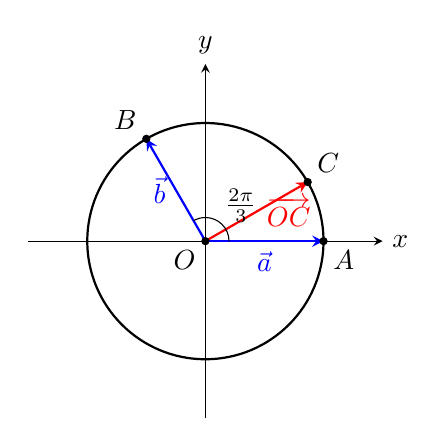
\begin{tikzpicture}[scale=1.5, >=stealth]
  \draw[->] (-1.5,0) -- (1.5,0) node[right] {\(x\)};
  \draw[->] (0,-1.5) -- (0,1.5) node[above] {\(y\)};
  \draw[thick] (0,0) circle (1);
  \coordinate (O) at (0,0);
  \coordinate (A) at (1,0);
  \coordinate (B) at (-0.5, 0.866);
  \coordinate (C) at (0.866, 0.5);
  
  \draw[->, thick, blue] (O) -- (A) node[midway, below] {\(\vec{a}\)};
  \draw[->, thick, blue] (O) -- (B) node[midway, left] {\(\vec{b}\)};
  \draw[->, thick, red] (O) -- (C) node[midway, right] {\(\overrightarrow{OC}\)};
  
  \fill (O) circle (1pt) node[below left] {\(O\)};
  \fill (A) circle (1pt) node[below right] {\(A\)};
  \fill (B) circle (1pt) node[above left] {\(B\)};
  \fill (C) circle (1pt) node[above right] {\(C\)};
  
  \draw (0.2,0) arc (0:120:0.2);
  \node at (0.3, 0.3) {\(\frac{2\pi}{3}\)};
\end{tikzpicture}
\end{center}

\teachblock{考点}{
非正交基底表示、二次约束下线性函数最值。}

\teachblock{读题切入口}{
令 \(\vec a=\vct{OA},\vec b=\vct{OB}\)，则
\[
|\vec a|=|\vec b|=1,\qquad \vec a\cdot\vec b=\cos\frac{2\pi}{3}=-\frac12.
\]
由 \(\vct{OC}=\lambda\vec a+\mu\vec b\) 且 \(C\) 在单位圆上，得到约束
\[
\lambda^2+\mu^2-\lambda\mu=1.
\]
}

\teachblock{解答}{
设
\[
r=\left(1+\frac{\sqrt3}{2},\,1\right),
\qquad
w=r_1\lambda+r_2\mu.
\]
约束对应的二次型为
\[
\lambda^2+\mu^2-\lambda\mu
=
\begin{bmatrix}\lambda&\mu\end{bmatrix}
\begin{bmatrix}1&-\frac12\\-\frac12&1\end{bmatrix}
\begin{bmatrix}\lambda\\ \mu\end{bmatrix}.
\]
在线性函数取最大值时，\((\lambda,\mu)\) 的方向与
\[
\begin{bmatrix}1&-\frac12\\-\frac12&1\end{bmatrix}^{-1}r
\]
同向。由于
\[
\begin{bmatrix}1&-\frac12\\-\frac12&1\end{bmatrix}^{-1}
=\frac43\begin{bmatrix}1&\frac12\\\frac12&1\end{bmatrix},
\]
故
\[
\lambda:\mu
=\left(1+\frac{\sqrt3}{2}+\frac12\right):
\left(\frac12+\frac{\sqrt3}{4}+1\right).
\]
因此
\[
\frac{\lambda}{\mu}
=\frac{\frac32+\frac{\sqrt3}{2}}{\frac32+\frac{\sqrt3}{4}}
=\frac{10+2\sqrt3}{11}.
\]
故选 \ans{C}。
}

\teachblock{方法点评}{
本题也可以用三角参数设 \(C=(\cos t,\sin t)\) 直接求 \(\lambda,\mu\)，再把 \(w\) 化成一个正弦型函数。讲评时可把二次型法作为培优方法，把参数法作为常规方法。
}

\section{多选题详细解析}

\subsection*{第 9 题：向量概念辨析}
关于平面向量，下列说法正确的是 (\quad) \\
A. 若 \(|\vec{a}|>|\vec{b}|\)，则 \(\vec{a}>\vec{b}\) \\
B. 若 \(\vec{a}=\vec{b}\)，则 \(\vec{a} \parallel \vec{b}\) \\
C. 若 \(\vec{a} \parallel \vec{b}, \vec{b} \parallel \vec{c}\)，则 \(\vec{a} \parallel \vec{c}\) \\
D. 若 \(\vec{a}=\vec{b}, \vec{b}=\vec{c}\)，则 \(\vec{a}=\vec{c}\)

\teachblock{考点}{
向量的相等、平行与大小比较。}

\teachblock{解答}{
\begin{enumerate}[label=\Alph*. , leftmargin=2em, itemsep=0.25em]
  \item 向量不能直接比较大小，\(|\vec a|>|\vec b|\) 只表示模长大小，不能写 \(\vec a>\vec b\)。错误。
  \item 若 \(\vec a=\vec b\)，则二者方向相同，故平行。正确。
  \item 若不排除零向量，\(\vec a\parallel \vec b,\vec b\parallel \vec c\) 不能推出 \(\vec a\parallel \vec c\)。例如 \(\vec b=\vec0\)，而 \(\vec a,\vec c\) 方向不同。错误。
  \item 向量相等具有传递性，正确。
\end{enumerate}
故选 \ans{BD}。
}

\teachblock{教学提醒}{
若某套教材对“零向量是否与任意向量平行”的约定不同，需要按教材口径处理。高考语境中通常要注意零向量造成的条件缺口。
}

\subsection*{第 10 题：三角函数图象读参题}
已知函数 \(f(x)=A\cos(\omega x+\varphi)\) (\(A>0, \omega>0, |\varphi|<\pi\)) 的部分图象如图所示，将函数 \(f(x)\) 的图象向左平移 \(\frac{\pi}{6}\) 个单位长度后得到 \(y=g(x)\) 的图象，则下列说法正确的是 (\quad) \\
A. \(\varphi=-\frac{5}{6}\pi\) \qquad
B. \(f(x+\frac{\pi}{3})=-f(-x+\frac{\pi}{3})\) \\
C. 函数 \(g(x)\) 为奇函数 \qquad
D. 函数 \(g(x)\) 在区间 \((\frac{5\pi}{12},\frac{3\pi}{4})\) 上单调递减


\begin{center}
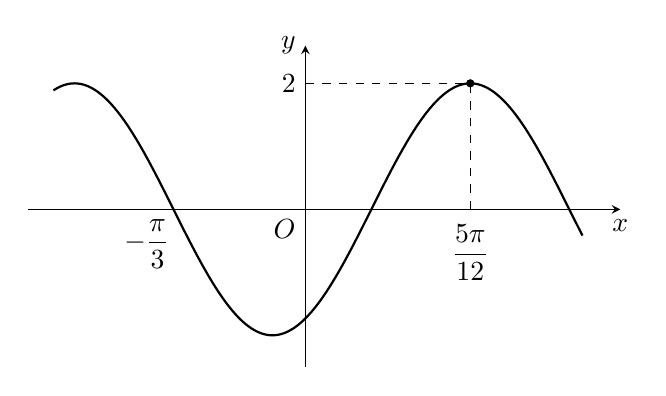
\begin{tikzpicture}[x=1.6cm, y=0.8cm, >=stealth]
  % Axes
  \draw[->] (-2.2,0) -- (2.5,0) node[below] {\(x\)};
  \draw[->] (0,-2.5) -- (0,2.6) node[left] {\(y\)};
  \node[below left] at (0,0) {\(O\)};
  
  % Plot function y = 2*cos(2*x - 150)
  \draw[thick, domain=-2.0:2.2, samples=100, smooth] 
    plot (\x, {2*cos(deg(2*\x - 5*3.1415926/6))});
    
  % Dashed lines for the peak (5pi/12, 2)
  \draw[dashed] (1.309, 0) -- (1.309, 2) -- (0, 2);
  
  % Tick labels
  \node[left] at (0,2) {\(2\)};
  \node[below, yshift=-2pt] at (1.309,0) {\(\dfrac{5\pi}{12}\)};
  \node[below left, xshift=2pt] at (-1.047,0) {\(-\dfrac{\pi}{3}\)};
  
  % Dots at key points
  \fill (1.309,2) circle (1.5pt);
\end{tikzpicture}
\end{center}

\teachblock{考点}{
三角函数图象读参、三角函数奇偶性、函数平移、单调性。
}

\teachblock{解答}{
对于 A：由图象可知最高点为 \(2\)，故 \(A=2\)。
从零点 \(x = -\dfrac{\pi}{3}\) 到相邻的最高点 \(x = \dfrac{5\pi}{12}\) 经历了 \(\dfrac{3}{4}\) 个周期，即：
\[
\frac{3}{4} T = \frac{5\pi}{12} - \left(-\frac{\pi}{3}\right) = \frac{3\pi}{4} \quad\Longrightarrow\quad T = \pi.
\]
so \(\omega = \dfrac{2\pi}{T} = 2\)。
代入最高点 \(\left(\dfrac{5\pi}{12}, \, 2\right)\) 得：
\[
2\cos\left(2\times \frac{5\pi}{12} + \varphi\right) = 2 \quad\Longrightarrow\quad \frac{5\pi}{6} + \varphi = 2k\pi \quad (k\in\mathbb{Z}).
\]
由 \(|\varphi| < \pi\) 解得 \(\varphi = -\dfrac{5\pi}{6}\)。
所以 \(f(x) = 2\cos\left(2x - \dfrac{5\pi}{6}\right)\)，选项 A 正确；

对于 B：因为 \(f\left(x+\dfrac{\pi}{3}\right) = 2\cos\left(2x - \dfrac{\pi}{6}\right)\)，而
\[
-f\left(-x+\dfrac{\pi}{3}\right) = -2\cos\left(-2x - \dfrac{\pi}{6}\right) = -2\cos\left(2x + \dfrac{\pi}{6}\right),
\]
二者不恒等（即 \(2\cos\left(2x - \dfrac{\pi}{6}\right) + 2\cos\left(2x + \dfrac{\pi}{6}\right) \not\equiv 0\)），故它不是奇函数，选项 B 错误；

对于 C：平移后得到：
\[
g(x) = 2\cos\left[2\left(x+\frac{\pi}{6}\right) - \frac{5\pi}{6}\right] = 2\cos\left(2x - \frac{\pi}{2}\right) = 2\sin 2x,
\]
显然为奇函数，选项 C 正确；

对于 D：当 \(x \in \left(\dfrac{5\pi}{12}, \, \dfrac{3\pi}{4}\right)\) 时，\(2x \in \left(\dfrac{5\pi}{6}, \, \dfrac{3\pi}{2}\right)\)。
由于 \(y = \sin x\) 在 \(\left(\dfrac{5\pi}{6}, \, \dfrac{3\pi}{2}\right)\) 上单调递减，所以 \(g(x) = 2\sin 2x\) 在区间 \(\left(\dfrac{5\pi}{12}, \, \dfrac{3\pi}{4}\right)\) 上单调递减，选项 D 正确。

故选 \ans{ACD}。
}

\teachblock{方法点评}{
图象读参题的核心在于读出关键点（最高点、最低点、零点），结合周期公式与相位范围求出解析式。判断平移后的性质时，应当小心括号内部的整体替换。
}

\subsection*{第 11 题：矩形折叠问题}
如图，矩形 \(ABCD\) 中，\(AB=2AD=2\)，\(E\) 为边 \(AB\) 的中点，将 \(\triangle ADE\) 沿直线 \(DE\) 翻折成 \(\triangle A_1DE\) (\(A_1 \notin\) 平面 \(BCDE\))，若 \(M\) 在线段 \(A_1C\) 上 (点 \(M\) 与 \(A_1, C\) 不重合)，则在 \(\triangle ADE\) 翻折过程中，给出下列判断，其中判断正确的有 (\quad) \\
A. 当 \(M\) 为 \(A_1C\) 的中点时，与平面 \(A_1DE\) 垂直的直线必与直线 \(MB\) 垂直 \\
B. 存在某个位置，使 \(DE \perp A_1C\) \\
C. 当四棱锥 \(A_1-BCDE\) 体积最大时，点 \(A_1\) 到平面 \(BCDE\) 的距离为 \(\frac{\sqrt{2}}{2}\) \\
D. 当二面角 \(A_1-DE-B\) 的大小为 \(\frac{\pi}{3}\) 时，异面直线 \(A_1D\) 与 \(BE\) 所成角的余弦值为 \(\frac{3}{4}\)

\begin{center}
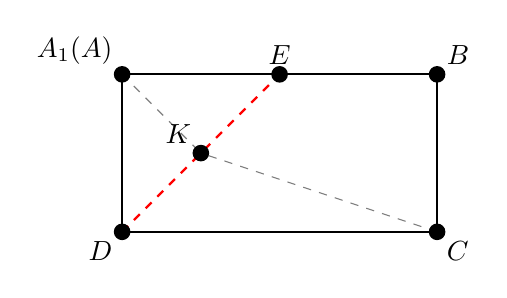
\begin{tikzpicture}[scale=2, >=stealth]
  % Coordinates of rectangle ABCD (AB=2, AD=1)
  \coordinate (D) at (0,0);
  \coordinate (C) at (2,0);
  \coordinate (B) at (2,1);
  \coordinate (A) at (0,1);
  \coordinate (E) at (1,1); % Midpoint of AB
  
  % Draw rectangle
  \draw[thick] (D) -- (C) -- (B) -- (A) -- cycle;
  
  % Fold line DE
  \draw[dashed, red, thick] (D) -- (E);
  
  % Midpoint K of DE
  \coordinate (K) at (0.5,0.5);
  
  % Connections
  \draw[dashed, gray] (A) -- (K);
  \draw[dashed, gray] (C) -- (K);
  
  % Dots
  \fill (D) circle (1.5pt) node[below left] {\(D\)};
  \fill (C) circle (1.5pt) node[below right] {\(C\)};
  \fill (B) circle (1.5pt) node[above right] {\(B\)};
  \fill (A) circle (1.5pt) node[above left] {\(A_1(A)\)};
  \fill (E) circle (1.5pt) node[above] {\(E\)};
  \fill (K) circle (1.5pt) node[above left] {\(K\)};
\end{tikzpicture}
\end{center}

\teachblock{考点}{
折叠不变量、二面角截面、线面垂直、体积最值、异面直线夹角。}

\teachblock{统一几何模型}{
矩形 \(ABCD\) 中 \(AB=2,AD=1\)，\(E\) 为 \(AB\) 中点。折痕为 \(DE\)。令 \(K\) 为 \(DE\) 的中点，则折叠过程中：
\[
A_1D=A_1E=1,\qquad DK=EK=\frac{\sqrt2}{2},\qquad A_1K=\frac{\sqrt2}{2},
\]
并且 \(A_1K\perp DE\)。点 \(A_1\) 绕直线 \(DE\) 旋转，其到平面 \(BCDE\) 的最大距离为 \(\dfrac{\sqrt2}{2}\)。
}

\teachblock{选项 A}{
设 \(H\) 为 \(A_1D\) 的中点。当 \(M\) 为 \(A_1C\) 的中点时，利用中点与矩形平行关系可得
\[
MB\parallel EH.
\]
而 \(EH\subset\) 平面 \(A_1DE\)，所以
\[
MB\parallel \text{平面 }A_1DE.
\]
于是任意垂直于平面 \(A_1DE\) 的直线，都与 \(MB\) 垂直。故 A 正确。
}

\teachblock{选项 B}{
因为 \(A_1K\perp DE\)，所以 \(A_1C\) 在 \(DE\) 方向上的分量只由 \(CK\) 决定。又在底面矩形中，\(CK\) 不垂直于 \(DE\)，因此无论如何折叠，都不可能有
\[
DE\perp A_1C.
\]
故 B 错误。
}

\teachblock{选项 C}{
四棱锥 \(A_1-BCDE\) 的底面 \(BCDE\) 固定，体积只随点 \(A_1\) 到平面 \(BCDE\) 的距离变化。点 \(A_1\) 绕折痕 \(DE\) 旋转，半径为
\[
A_1K=\frac{\sqrt2}{2}.
\]
当平面 \(A_1DE\perp\) 平面 \(BCDE\) 时，高最大，最大高为
\[
\frac{\sqrt2}{2}.
\]
故 C 正确。
}

\teachblock{选项 D}{
设异面直线 \(A_1D\) 与 \(BE\) 的夹角为 \(\theta\)。设 \(K\) 为 \(DE\) 的中点，过 \(K\) 作垂直于 \(DE\) 的截面。令折叠参数 \(t\) 满足 \(\overrightarrow{KA_1}=\frac{\sqrt2}{2}(\cos t\,\vec e+\sin t\,\vec n)\)，其中 \(\vec e\) 为底面内垂直于 \(DE\) 的单位方向，\(\vec n\) 为底面法向量。

由于 \(BE\) 与矩形边 \(AB\) 同向，计算 \(A_1D\) 在 \(BE\) 方向上的投影，可得
\[
\cos\angle(A_1D,BE)=\frac{1-\cos t}{2}.
\]
又二面角 \(A_1-DE-B=\frac{\pi}{3}\) 对应截面内 \(\angle A_1KB=\frac{\pi}{3}\)，而 \(KB\) 在截面内与初始 \(KA\) 反向，所以 \(-\cos t=\frac12\)，即 \(\cos t=-\frac12\)。
于是
\[
\cos\angle(A_1D,BE)=\frac{1-\left(-\frac12\right)}{2}=\frac34.
\]
故 D 正确。
}

\teachblock{结论}{
本题正确选项为 \ans{ACD}。
}

\teachblock{教学主线}{
这道折叠题要反复强调：折叠不是“凭空间感觉猜”，而是“绕折痕旋转”。所有判断都先找折痕 \(DE\)，再找垂足 \(K\)，再转化为垂直截面或固定底面上的距离问题。
}

\section{填空题详细解析}

\subsection*{第 12 题：分层抽样估计}
某校高一共有学生 800 人，现采用分层抽样的方法从中抽取 80 人进行体能测试，若这 80 人中有 39 人是男生，据此估计该校高一男生有 \_\_\_\_\_\_\_ 人。

\teachblock{解答}{
样本中男生比例为
\[
\frac{39}{80}.
\]
据此估计全体 800 人中的男生人数为
\[
800\cdot\frac{39}{80}=390.
\]
答案：\ans{390}。
}

\teachblock{方法点评}{
分层抽样估计题抓住“样本比例约等于总体比例”。}

\subsection*{第 13 题：诱导公式与二倍角}
已知 \(\sin\alpha=\frac{\sqrt{5}}{5}\)，则 \(\sin(2\alpha-\frac{\pi}{2})=\) \_\_\_\_\_\_\_。

\teachblock{解答}{
\[
\sin\left(2\alpha-\frac{\pi}{2}\right)=-\cos2\alpha.
\]
又
\[
\cos2\alpha=1-2\sin^2\alpha
=1-2\cdot\frac15=\frac35.
\]
所以
\[
\sin\left(2\alpha-\frac{\pi}{2}\right)=-\frac35.
\]
答案：\ans{-\dfrac35}。
}

\teachblock{易错提醒}{
本题不需要知道 \(\alpha\) 的象限，因为 \(\cos2\alpha\) 可直接由 \(\sin^2\alpha\) 确定。
}

\subsection*{第 14 题：正四棱台与外接球}
正四棱台 \(ABCD-A_1B_1C_1D_1\) 的体积为 \(\frac{304}{3}\)，上底面 \(A_1B_1C_1D_1\)，下底面 \(ABCD\) 的边长分别为 4, 6，记 \(AC, BD\) 交于点 \(O\)，\(A_1C_1, B_1D_1\) 交于点 \(O_1\)，则 \(OA_1=\) \_\_\_\_\_\_\_；若四棱台 \(ABCD-A_1B_1C_1D_1\) 的各个顶点均在球 \(O_2\) 的表面上，则球 \(O_2\) 的表面积为 \_\_\_\_\_\_\_。

\begin{center}
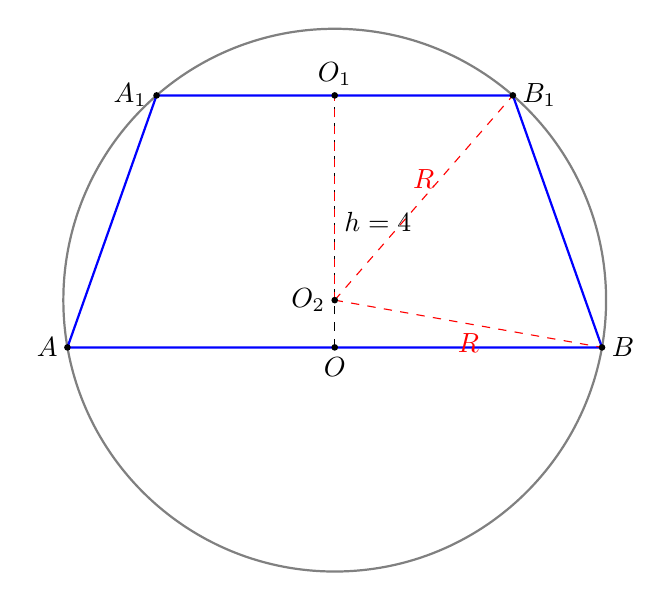
\begin{tikzpicture}[scale=0.8, >=stealth]
  % Coordinates of axis section
  % Sphere center is at (0, 0.75) relative to bottom base center
  \coordinate (O) at (0,0); % bottom base center
  \coordinate (O1) at (0,4); % top base center
  \coordinate (O2) at (0,0.75); % Sphere center
  
  % Radius is R = sqrt(297)/4 = 4.308
  \draw[thick, gray] (O2) circle (4.308);
  
  % Vertices of trapezoid
  \coordinate (A) at (-4.243, 0); % 3*sqrt(2)
  \coordinate (B) at (4.243, 0);
  \coordinate (A1) at (-2.828, 4); % 2*sqrt(2)
  \coordinate (B1) at (2.828, 4);
  
  % Draw axis section trapezoid
  \draw[thick, blue] (A) -- (B) -- (B1) -- (A1) -- cycle;
  
  % Draw vertical axis
  \draw[dashed] (O) -- (O1);
  
  % Draw sphere radius lines
  \draw[dashed, red] (O2) -- (B) node[midway, below] {\(R\)};
  \draw[dashed, red] (O2) -- (B1) node[midway, above] {\(R\)};
  \draw[dashed, red] (O2) -- (O1);
  
  % Dots
  \fill (O) circle (1.5pt) node[below] {\(O\)};
  \fill (O1) circle (1.5pt) node[above] {\(O_1\)};
  \fill (O2) circle (1.5pt) node[left] {\(O_2\)};
  \fill (A) circle (1.5pt) node[left] {\(A\)};
  \fill (B) circle (1.5pt) node[right] {\(B\)};
  \fill (A1) circle (1.5pt) node[left] {\(A_1\)};
  \fill (B1) circle (1.5pt) node[right] {\(B_1\)};
  
  % Labels
  \node[right] at (0, 2) {\(h=4\)};
\end{tikzpicture}
\end{center}

\teachblock{考点}{
棱台体积、轴截面、外接球球心位置。}

\teachblock{解答}{
正四棱台上下底面边长分别为 \(6,4\)，面积分别为 \(36,16\)。设高为 \(h\)，则
\[
V=\frac{h}{3}(36+16+\sqrt{36\cdot16})
=\frac{h}{3}(36+16+24)=\frac{76h}{3}.
\]
由
\[
\frac{76h}{3}=\frac{304}{3}
\]
得
\[
h=4.
\]

设上下底面中心分别为 \(O,O_1\)，则 \(OO_1=4\)，且
\[
O_1A_1=\frac{4\sqrt2}{2}=2\sqrt2.
\]
于是
\[
OA_1=\sqrt{OO_1^2+O_1A_1^2}
=\sqrt{4^2+(2\sqrt2)^2}=2\sqrt6.
\]

外接球球心 \(O_2\) 在轴 \(OO_1\) 上。设 \(OO_2=t\)，球半径为 \(R\)。下底面顶点到轴的距离为 \(3\sqrt2\)，上底面顶点到轴的距离为 \(2\sqrt2\)，故
\[
R^2=18+t^2=8+(4-t)^2.
\]
解得
\[
t=\frac34,\qquad R^2=18+\frac{9}{16}=\frac{297}{16}.
\]
球的表面积为
\[
4\pi R^2=\frac{297\pi}{4}.
\]
答案：\ans{2\sqrt6,\ \dfrac{297\pi}{4}}。
}

\teachblock{方法点评}{
正棱台外接球问题的主线是“球心在对称轴上”。不要在空间中乱找球心，先用对称性降维到轴截面。
}

\section{解答题详细解析}

\subsection*{第 15 题：复数的实部虚部与象限}
已知复数 \(z_1=(m+1)+mi, z_2=1+i\)，其中 \(m \in \mathbb{R}\)，\(i\) 为虚数单位。\\
(1) 若复数 \(z_1 \cdot z_2\) 为实数，求实数 \(m\) 的值；\\
(2) 在复平面内，若复数 \(z=z_1+\sqrt{2}|z_2|\) 对应的点在第一象限，求实数 \(m\) 的取值范围。

\teachblock{考点}{
复数乘法、实数条件、复平面象限。}

\teachblock{第（1）问}{
\[
z_1z_2=[(m+1)+mi](1+i)
=(m+1-m)+(m+1+m)i
=1+(2m+1)i.
\]
若 \(z_1z_2\) 为实数，则虚部为 \(0\)，即
\[
2m+1=0,\qquad m=-\frac12.
\]
}

\teachblock{第（2）问}{
因为
\[
|z_2|=|1+i|=\sqrt2,
\]
所以
\[
\sqrt2|z_2|=2.
\]
于是
\[
z=z_1+\sqrt2|z_2|
=(m+1)+mi+2=(m+3)+mi.
\]
复数对应点在第一象限，要求
\[
m+3>0,\qquad m>0.
\]
故
\[
m>0.
\]
}

\teachblock{卷面规范}{
第一象限必须同时写出实部、虚部两个不等式，不能只写 \(m>0\) 而没有说明实部条件。
}

\subsection*{第 16 题：四棱锥中的平行与线面角}
在四棱锥 \(P-ABCD\) 中，底面 \(ABCD\) 是边长为 2 的菱形，\(\angle DAB=60^\circ\)，\(\triangle PAD\) 是以 \(PA\) 为斜边的等腰直角三角形，\(\triangle PCD\) 是以 \(PC\) 为斜边的等腰直角三角形，\(F, G, H\) 分别是 \(PB, CD, PA\) 的中点。\\
(1) 求证：\(GF \parallel\) 平面 \(PAD\)；\\
(2) 求直线 \(PB\) 与平面 \(ABCD\) 所成角。

\begin{center}
\begin{tikzpicture}[>=stealth, scale=1.5]
  % Define coordinates
  \coordinate (D) at (0,0);
  \coordinate (C) at (2.0,0);
  \coordinate (A) at (-0.8,-0.8);
  \coordinate (B) at (1.2,-0.8);
  \coordinate (P) at (0,2.2);
  
  % Midpoints
  \coordinate (G) at ($(C)!0.5!(D)$);
  \coordinate (F) at ($(P)!0.5!(B)$);
  \coordinate (H) at ($(P)!0.5!(A)$);
  
  % Draw dashed lines (back)
  \draw[dashed, gray, thick] (D) -- (A);
  \draw[dashed, gray, thick] (D) -- (C);
  \draw[dashed, gray, thick] (P) -- (D);
  \draw[dashed, gray, thick] (G) -- (F);
  \draw[dashed, gray, thick] (D) -- (H);
  
  % Draw solid lines (front)
  \draw[thick] (P) -- (A) -- (B) -- (C) -- (P) -- (B);
  \draw[thick] (A) -- (B);
  
  % Labels
  \node[above] at (P) {\(P\)};
  \node[left] at (D) {\(D\)};
  \node[right] at (C) {\(C\)};
  \node[below left] at (A) {\(A\)};
  \node[below right] at (B) {\(B\)};
  \node[above right, scale=0.8] at (G) {\(G\)};
  \node[right, scale=0.8] at (F) {\(F\)};
  \node[left, scale=0.8] at (H) {\(H\)};
\end{tikzpicture}
\end{center}

\teachblock{考点}{
中位线、线面平行判定、线面角。}

\teachblock{关键结构}{
底面 \(ABCD\) 是边长为 \(2\) 的菱形，且 \(\angle DAB=60^\circ\)。因此 \(BD=2\)。

\(\triangle PAD\) 是以 \(PA\) 为斜边的等腰直角三角形，所以
\[
PD\perp AD,\qquad PD=AD=2.
\]
\(\triangle PCD\) 是以 \(PC\) 为斜边的等腰直角三角形，所以
\[
PD\perp CD,\qquad PD=CD=2.
\]
由于 \(AD,CD\) 是底面内两条相交直线，故
\[
PD\perp \text{平面 }ABCD.
\]
}

\teachblock{第（1）问：证明 \(GF\parallel\) 平面 \(PAD\)}{
设 \(H\) 为 \(PA\) 的中点。因为 \(F,H\) 分别为 \(PB,PA\) 的中点，所以在 \(\triangle PAB\) 中
\[
FH\parallel AB,\qquad FH=\frac12AB.
\]
又 \(G\) 为 \(CD\) 的中点，故
\[
DG=\frac12CD.
\]
菱形中 \(AB\parallel CD\) 且 \(AB=CD\)，于是
\[
FH\parallel DG,\qquad FH=DG.
\]
所以四边形 \(DGFH\) 为平行四边形，从而
\[
GF\parallel DH.
\]
而 \(D,H\) 均在平面 \(PAD\) 内，所以 \(DH\subset\) 平面 \(PAD\)。又 \(GF\) 不在平面 \(PAD\) 内，故
\[
GF\parallel \text{平面 }PAD.
\]
}

\teachblock{第（2）问：求直线 \(PB\) 与平面 \(ABCD\) 所成角}{
由上已知 \(PD\perp\) 平面 \(ABCD\)，所以 \(PB\) 在底面上的射影为 \(DB\)。因此直线 \(PB\) 与平面 \(ABCD\) 所成角为
\[
\angle PBD.
\]
在直角三角形 \(PDB\) 中，
\[
PD=2,\qquad DB=2.
\]
故
\[
\tan\angle PBD=\frac{PD}{DB}=1,
\]
从而
\[
\angle PBD=\frac{\pi}{4}.
\]
}

\teachblock{教学点评}{
此题应避免一开始坐标化。第（1）问的核心是“补中点 \(H\)，造平行四边形”；第（2）问的核心是先证明 \(PD\perp\) 底面，再在直角三角形 \(PDB\) 中计算。
}

\subsection*{第 17 题：解三角形与中线}
在 \(\triangle ABC\) 中，内角 \(A, B, C\) 对应的边分别是 \(a, b, c\)，且 \(b\cos C+c\cos B=2a\cos A\)。\\
(1) 求角 \(A\)；\\
(2) 若 \(AB\) 的长为 3，\(AC\) 边上的中线 \(BD\) 长为 \(\sqrt{7}\)，求 \(\triangle ABC\) 的周长。

\begin{center}
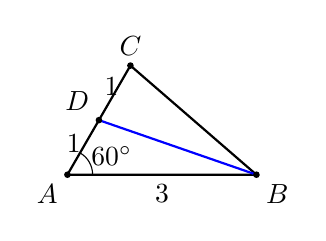
\begin{tikzpicture}[scale=0.8, >=stealth]
  \coordinate (A) at (0,0);
  \coordinate (B) at (3,0);
  \coordinate (C1) at (1, 1.732);
  \coordinate (D1) at (0.5, 0.866);
  
  \draw[thick] (A) -- (B) -- (C1) -- cycle;
  \draw[thick, blue] (B) -- (D1);
  
  \fill (A) circle (1.5pt) node[below left] {\(A\)};
  \fill (B) circle (1.5pt) node[below right] {\(B\)};
  \fill (C1) circle (1.5pt) node[above] {\(C\)};
  \fill (D1) circle (1.5pt) node[above left] {\(D\)};
  
  \node at (1.5, -0.3) {\(3\)};
  \node at (0.1, 0.5) {\(1\)};
  \node at (0.7, 1.4) {\(1\)};
  
  \draw (0.4,0) arc (0:60:0.4);
  \node at (0.7, 0.3) {\(60^\circ\)};
\end{tikzpicture}
\qquad
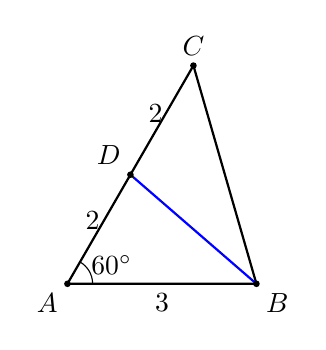
\begin{tikzpicture}[scale=0.8, >=stealth]
  \coordinate (A) at (0,0);
  \coordinate (B) at (3,0);
  \coordinate (C2) at (2, 3.464);
  \coordinate (D2) at (1, 1.732);
  
  \draw[thick] (A) -- (B) -- (C2) -- cycle;
  \draw[thick, blue] (B) -- (D2);
  
  \fill (A) circle (1.5pt) node[below left] {\(A\)};
  \fill (B) circle (1.5pt) node[below right] {\(B\)};
  \fill (C2) circle (1.5pt) node[above] {\(C\)};
  \fill (D2) circle (1.5pt) node[above left] {\(D\)};
  
  \node at (1.5, -0.3) {\(3\)};
  \node at (0.4, 1.0) {\(2\)};
  \node at (1.4, 2.7) {\(2\)};
  
  \draw (0.4,0) arc (0:60:0.4);
  \node at (0.7, 0.3) {\(60^\circ\)};
\end{tikzpicture}
\end{center}

\teachblock{考点}{
边角互化、余弦定理、中线长公式。}

\teachblock{第（1）问：求角 \(A\)}{
由余弦定理的投影形式：
\[
b\cos C+c\cos B=a.
\]
原式给出
\[
b\cos C+c\cos B=2a\cos A,
\]
所以
\[
a=2a\cos A.
\]
由于 \(a>0\)，故
\[
\cos A=\frac12,\qquad A=\frac{\pi}{3}.
\]
}

\teachblock{第（2）问：求周长}{
在 \(\triangle ABD\) 中，已知 \(AB=3\)，\(BD=\sqrt7\)，由余弦定理得：
\[
BD^2 = AB^2 + AD^2 - 2AB\cdot AD\cos A.
\]
代入数据得：
\[
7 = 9 + AD^2 - 2\cdot 3\cdot AD\cdot \frac{1}{2} \quad\Longrightarrow\quad AD^2 - 3AD + 2 = 0.
\]
解得 \(AD=1\) 或 \(AD=2\)。

因为 \(D\) 为 \(AC\) 的中点，所以：
\begin{itemize}
  \item 当 \(AD=1\) 时，\(AC=2\)。在 \(\triangle ABC\) 中，由余弦定理得：
  \[
  BC^2 = AB^2 + AC^2 - 2AB\cdot AC\cos A = 9 + 4 - 2\cdot 3\cdot 2\cdot \frac{1}{2} = 7.
  \]
  所以 \(BC=\sqrt7\)，此时 \(\triangle ABC\) 的周长为 \(3 + 2 + \sqrt7 = 5+\sqrt7\)。
  
  \item 当 \(AD=2\) 时，\(AC=4\)。在 \(\triangle ABC\) 中，由余弦定理得：
  \[
  BC^2 = AB^2 + AC^2 - 2AB\cdot AC\cos A = 9 + 16 - 2\cdot 3\cdot 4\cdot \frac{1}{2} = 13.
  \]
  so \(BC=\sqrt{13}\)，此时 \(\triangle ABC\) 的周长为 \(3 + 4 + \sqrt{13} = 7+\sqrt{13}\)。
\end{itemize}
综上所述，\(\triangle ABC\) 的周长为 \(5+\sqrt7\) 或 \(7+\sqrt{13}\)。
}

\begin{warnbox}{命题提示}
两组结果均满足三角形条件与题设。标准答案也确实保留了这两个答案，说明本题有双解。
\end{warnbox}

\subsection*{第 18 题：正方体中的展开、垂直与二面角范围}
在正方体 \(ABCD-A_1B_1C_1D_1\) 中，\(AB=2, E\) 是棱 \(C_1D_1\) 的中点，\(F\) 是正方体棱上的一动点。\\
(1) 若 \(F\) 为线段 \(A_1D_1\) 上的动点，求 \(AF+FE\) 的最小值；\\
(2) 证明：平面 \(AA_1C_1C \perp\) 平面 \(BC_1D\)；\\
(3) 若 \(F\) 为线段 \(A_1E\) 上的动点，求平面 \(ABF\) 与平面 \(CDF\) 夹角的余弦值的取值范围。

\begin{center}
\begin{tikzpicture}[scale=1.5, >=stealth]
  % Define 3D coordinates for cube
  \coordinate (D) at (0,0);
  \coordinate (C) at (2,0);
  \coordinate (A) at (-0.8,-0.8);
  \coordinate (B) at (1.2,-0.8);
  
  \coordinate (D1) at (0,2);
  \coordinate (C1) at (2,2);
  \coordinate (A1) at (-0.8,1.2);
  \coordinate (B1) at (1.2,1.2);
  
  % Midpoints
  \coordinate (E) at ($(C1)!0.5!(D1)$);
  \coordinate (F) at ($(A1)!0.6!(D1)$); % F on A1D1
  
  % Dashed lines (back/inside)
  \draw[dashed, gray] (D) -- (C);
  \draw[dashed, gray] (D) -- (A);
  \draw[dashed, gray] (D) -- (D1);
  \draw[dashed, gray] (A) -- (C); % AC
  
  % Solid lines (front/outside)
  \draw[thick] (A) -- (B) -- (C) -- (C1) -- (D1) -- (A1) -- cycle;
  \draw[thick] (B) -- (B1);
  \draw[thick] (A1) -- (B1) -- (C1);
  
  % Path A -> F -> E
  \draw[thick, blue] (A) -- (F) -- (E);
  
  % Labels
  \node[left] at (D) {\(D\)};
  \node[right] at (C) {\(C\)};
  \node[below left] at (A) {\(A\)};
  \node[below right] at (B) {\(B\)};
  \node[above left] at (D1) {\(D_1\)};
  \node[above right] at (C1) {\(C_1\)};
  \node[left] at (A1) {\(A_1\)};
  \node[right] at (B1) {\(B_1\)};
  \node[above, blue] at (E) {\(E\)};
  \node[above left, blue] at (F) {\(F\)};
\end{tikzpicture}
\quad
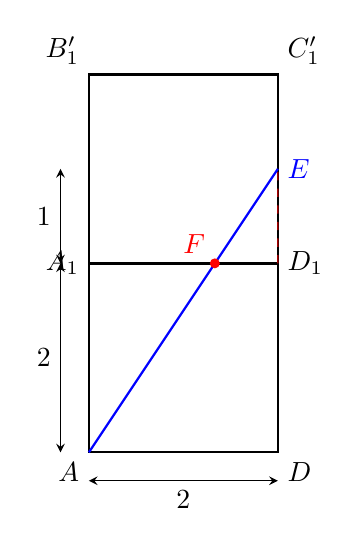
\begin{tikzpicture}[scale=1.2, >=stealth]
  % Draw side face ADD1A1
  \draw[thick] (0,0) rectangle (2,2);
  % Draw top face A1B1C1D1 unfolded
  \draw[thick] (0,2) rectangle (2,4);
  
  % Coordinates
  \coordinate (A) at (0,0);
  \coordinate (D) at (2,0);
  \coordinate (A1) at (0,2);
  \coordinate (D1) at (2,2);
  \coordinate (B1) at (0,4);
  \coordinate (C1) at (2,4);
  \coordinate (E) at (2,3); % Midpoint of D1C1 in unfolded view
  
  % Path
  \draw[thick, blue] (A) -- (E);
  \draw[dashed, red] (2,2) -- (E);
  
  % Labels
  \node[below left] at (A) {\(A\)};
  \node[below right] at (D) {\(D\)};
  \node[left] at (A1) {\(A_1\)};
  \node[right] at (D1) {\(D_1\)};
  \node[above left] at (B1) {\(B_1'\)};
  \node[above right] at (C1) {\(C_1'\)};
  \node[right, blue] at (E) {\(E\)};
  
  % Dimensions
  \draw[<->] (-0.3,0) -- (-0.3,2) node[midway, left] {\(2\)};
  \draw[<->] (-0.3,2) -- (-0.3,3) node[midway, left] {\(1\)};
  \draw[<->] (0,-0.3) -- (2,-0.3) node[midway, below] {\(2\)};
  
  % Point F
  \coordinate (F) at (1.333,2);
  \fill[red] (F) circle (1.5pt) node[above left] {\(F\)};
\end{tikzpicture}
\end{center}

\teachblock{考点}{
立方体展开最短路、面面垂直、平面夹角取值范围。}

\teachblock{第（1）问：求 \(AF+FE\) 的最小值}{
点 \(F\) 在线段 \(A_1D_1\) 上。路径 \(A\to F\to E\) 分别位于侧面 \(ADD_1A_1\) 与顶面 \(A_1B_1C_1D_1\) 上，可沿公共边 \(A_1D_1\) 展开。

在展开图中，\(A\) 到边 \(A_1D_1\) 的垂直距离为 \(2\)，\(E\) 到边 \(A_1D_1\) 的垂直距离为 \(1\)，二者在边方向上的距离为 \(2\)。最短折线化为一条直线，因此
\[
(AF+FE)_{\min}
=\sqrt{2^2+(2+1)^2}
=\sqrt{13}.
\]
}

\teachblock{第（2）问：证明两个平面垂直}{
在正方体底面正方形 \(ABCD\) 中，
\[
BD\perp AC.
\]
又 \(BD\perp AA_1\)，且 \(AC,AA_1\) 是平面 \(AA_1C_1C\) 内两条相交直线，所以
\[
BD\perp \text{平面 }AA_1C_1C.
\]
而
\[
BD\subset \text{平面 }BC_1D.
\]
因此
\[
\text{平面 }AA_1C_1C\perp \text{平面 }BC_1D.
\]
}

\teachblock{第（3）问：求夹角余弦值范围}{
【几何降维分析】由于 \(AB\parallel CD\)，两平面分别含有平行直线，所以可取垂直于 \(AB\) 的截面来求夹角。截面分别交两个平面于两条直线，这两条直线的夹角就是二面角，然后在二维内转化为参数计算。

【具体计算】设正方体棱长为 \(2\)。令 \(F\) 在线段 \(A_1E\) 上运动，用参数 \(t\in[0,1]\) 表示：
\[
A_1F:tFE=t:(1-t).
\]
沿三条互相垂直的棱方向作长度分解，可取
\[
F=(t,2t,2).
\]
平面 \(ABF\) 可取一个法向量
\[
\vec n_1=(0,-1,t),
\]
平面 \(CDF\) 可取一个法向量
\[
\vec n_2=(0,1,1-t).
\]
故两平面夹角 \(\theta\) 的余弦值为
\[
\cos\theta
=\frac{|\vec n_1\cdot\vec n_2|}{|\vec n_1||\vec n_2|}
=\frac{t^2-t+1}{\sqrt{(1+t^2)\left(1+(1-t)^2\right)}}.
\]
令
\[
u=t(1-t),\qquad 0\leq u\leq\frac14.
\]
则
\[
\cos\theta
=\frac{1-u}{\sqrt{(1-u)^2+1}}.
\]
该式随 \(1-u\) 增大而增大，而
\[
1-u\in\left[\frac34,1\right].
\]
所以
\[
\cos\theta\in
\left[
\frac{\frac34}{\sqrt{\frac{9}{16}+1}},
\frac{1}{\sqrt2}
\right]
=
\left[\frac35,\frac{\sqrt2}{2}\right].
\]
}

\teachblock{教学点评}{
第（1）（2）问建议坚持纯几何：展开图和垂直判定最清楚。第（3）问若强行纯几何会很长，课堂上可以说明“此处是平面角范围问题，适度引入法向量是为了把动态几何量降为单变量函数”。
}

\subsection*{第 19 题：新定义函数与几何存在性}
已知在平面直角坐标系中，\(O\) 为坐标原点，定义函数 \(f(x)=p\sin x+q\cos x\) 的“和谐向量”为非零向量 \(\vec{\omega}=(p,q)\)，\(\vec{\omega}=(p,q)\) 的“和谐函数”为 \(f(x)=p\sin x+q\cos x\)。记平面内所有向量的“和谐函数”构成的集合为 \(T\)。\\
(1) 已知 \(\theta \in \mathbf{R}\)，\(f(x)=2\sin x+\sin(x+\theta)\)，若函数 \(f(x)\) 为集合 \(T\) 中的元素，求其“和谐向量”模的取值范围；\\
(2) 已知 \(|\vec{a}|=|\vec{b}|=3\)，设 \(\overrightarrow{OG}=\lambda\vec{a}+\mu\vec{b}\) (\(\lambda>0, \mu>0\))，且 \(\overrightarrow{OG}\) 的“和谐函数”为 \(\varphi(x)\)，其最大值为 \(S\)，求 \(\frac{\lambda+\mu}{S}\)；\\
(3) 已知 \(M(-2,3), N(2,6)\)，设(1)中的“和谐函数”的模取得最小时的“和谐函数”为 \(m(x)\)，\(g(x)=2m(\frac{x}{2})\)，试问在 \(y=g(x)\) 的图象上是否存在一点 \(Q\)，使得 \(\overrightarrow{MQ} \cdot \overrightarrow{NQ}=0\)，若存在，求出 \(Q\) 点坐标；若不存在，说明理由。

\teachblock{考点}{
新定义阅读、正弦型函数振幅、向量模、圆与函数图象交点。}

\teachblock{第（1）问：求和谐向量模的取值范围}{
\[
f(x)=2\sin x+\sin(x+\theta)
=2\sin x+\sin x\cos\theta+\cos x\sin\theta.
\]
所以其“和谐向量”为
\[
\vec\omega=(2+\cos\theta,\ \sin\theta).
\]
模为
\[
|\vec\omega|
=\sqrt{(2+\cos\theta)^2+\sin^2\theta}
=\sqrt{5+4\cos\theta}.
\]
因为 \(\cos\theta\in[-1,1]\)，所以
\[
|\vec\omega|\in[1,3].
\]
}

\teachblock{第（2）问：原题条件不足}{
在原题条件下，\(\frac{\lambda+\mu}{S}\) 不能唯一确定。给出两个反例：
\begin{itemize}
    \item 若 \(\vec a=\vec b\)，则 \(S=3(\lambda+\mu)\)，所以 \(\frac{\lambda+\mu}{S}=\frac13\)。
    \item 若 \(\vec a\perp \vec b\)，取 \(\lambda=\mu=1\)，则 \(S=|\overrightarrow{OG}|=3\sqrt2\)，所以 \(\frac{\lambda+\mu}{S}=\frac{2}{3\sqrt2}=\frac{\sqrt2}{3}\)。
\end{itemize}
两个结果不同，因此原题缺少条件。这也锻炼了学生的命题审查意识。
}
\teachblock{原标准答案（默认 $\vec a=\vec b$ 同向的推导）}{
设 \(\vec a = (3\cos\alpha, 3\sin\alpha)\)，\(\vec b = (3\cos\beta, 3\sin\beta)\)，由 \(\vec{OG} = \lambda\vec a + \mu\vec b\)，得：
\[
\vec{OG} = \left( 3(\lambda\cos\alpha + \mu\cos\beta), \, 3(\lambda\sin\alpha + \mu\sin\beta) \right).
\]
根据定义，\(\vec{OG}\) 的“和谐函数”为 \(\varphi(x)\)：
\[
\begin{aligned}
\varphi(x) &= 3(\lambda\cos\alpha + \mu\cos\beta)\sin x + 3(\lambda\sin\alpha + \mu\sin\beta)\cos x \\
&= 3\lambda(\sin x\cos\alpha + \cos x\sin\alpha) + 3\mu(\sin x\cos\beta + \cos x\sin\beta) \\
&= 3\lambda\sin(x+\alpha) + 3\mu\sin(x+\beta).
\end{aligned}
\]
因为 \(\sin(x+\alpha) \le 1\)，\(\sin(x+\beta) \le 1\)，且 \(\lambda > 0\)，\(\mu > 0\)，所以：
\[
\varphi(x) \le 3\lambda + 3\mu.
\]
当且仅当存在 \(x_0\) 满足：
\[
\begin{cases}
x_0 + \alpha = \dfrac{\pi}{2} + 2k_1\pi, \\
x_0 + \beta = \dfrac{\pi}{2} + 2k_2\pi
\end{cases} \quad (k_1, k_2 \in \mathbb{Z})
\]
时，等号成立。此时由两式相减得：
\[
\alpha - \beta = 2(k_1 - k_2)\pi \quad\Longrightarrow\quad \vec a = \vec b.
\]
所以，若 \(\varphi(x)\) 能取到其最大可能上界，则必须 \(\vec a = \vec b\)，此时最大值为：
\[
S = 3\lambda + 3\mu.
\]
从而：
\[
\frac{\lambda + \mu}{S} = \frac{1}{3}.
\]
}

\teachblock{第（3）问：判断点 \(Q\) 是否存在}{
由第（1）问知，当 \(\cos\theta = -1\) 时，\(|\vec\omega|\) 最小，此时 \(\vec\omega = (1, 0)\)。
则对应的和谐函数为 \(m(x) = \sin x\)，所以：
\[
g(x) = 2m\left(\frac{x}{2}\right) = 2\sin\frac{x}{2}.
\]

【圆与函数图象法（更优）】
由 \(\overrightarrow{MQ}\cdot\overrightarrow{NQ}=0\) 可知 \(\angle MQN=90^\circ\)，所以 \(Q\) 在以 \(MN\) 为直径的圆上。
已知 \(M(-2,3), N(2,6)\)，圆心为 \(\left(0,\frac92\right)\)，半径为 \(R=\frac{MN}{2}=\frac52\)。
所以该圆的最低点纵坐标为 \(\frac92-\frac52=2\)。
而点 \(Q\) 在函数 \(g(x)=2\sin\frac{x}{2}\) 的图象上，且 \(g(x)\le 2\)。
因此若圆与函数图象有交点，只可能在圆的最低点 \(Q=(0,2)\)。
但 \(g(0)=0\ne 2\)，所以不存在这样的点 \(Q\)。此解法比纯代数配方更清爽。

\begin{center}
\begin{tikzpicture}[scale=0.8, >=stealth]
  \draw[->] (-3,0) -- (8,0) node[below] {\(x\)};
  \draw[->] (0,-1) -- (0,8) node[left] {\(y\)};
  
  \coordinate (M) at (-2,3);
  \coordinate (N) at (2,6);
  \coordinate (Center) at (0,4.5);
  
  \fill (M) circle (1.5pt) node[left] {\(M(-2,3)\)};
  \fill (N) circle (1.5pt) node[right] {\(N(2,6)\)};
  \fill (Center) circle (1.5pt) node[right] {\((0,4.5)\)};
  
  \draw[thick, blue] (Center) circle (2.5);
  \draw[dashed] (M) -- (N);
  
  \draw[thick, red, domain=-3:8, samples=100] plot (\x, {2*sin(deg(\x/2))});
  
  \coordinate (Lowest) at (0,2);
  \fill (Lowest) circle (1.5pt) node[above right] {\((0,2)\)};
  
  \node[red, right] at (6.28, 0.5) {\(y=2\sin\frac{x}{2}\)};
\end{tikzpicture}
\end{center}
}

\teachblock{教学点评}{
新定义题的第一步不是“害怕定义”，而是把定义翻译成旧知识：这里的“和谐函数最大值”就是向量 \((p,q)\) 的模。第（3）问则转化为“直径为 \(MN\) 的圆与函数图象是否相交”。
}

\newpage

\section{讲评课主线建议}

\begin{teachbox}{建议讲评顺序}
若本卷用于 90--120 分钟讲评课，不建议完全按题号推进。可以按以下主线组织：
\begin{enumerate}[label=\arabic*. , leftmargin=2em, itemsep=0.25em]
  \item 基础快讲：1、2、4、12、13、15，用于稳定复数、坐标、向量、抽样与三角基本功。
  \item 方法精讲：3、7、8、17、19，重点讲“条件翻译、分类讨论、参数或约束最值、新定义阅读”。
  \item 立体几何专题讲：6、11、16、18，按“中点与平移、折叠不变量、线面垂直、展开最短路、面面垂直”串成一条线。
  \item 命题校对与审题提醒：10、17、19(2)，告诉学生不是所有题都能在缺条件时硬算，审题与质疑也是数学能力。
\end{enumerate}
\end{teachbox}

\begin{keybox}{本卷核心方法沉淀}
\begin{enumerate}[label=\arabic*. , leftmargin=2em, itemsep=0.25em]
  \item \textbf{复数题先化标准形}：先写成 \(a+bi\)，再判断模、实数、象限。
  \item \textbf{向量题注意零向量}：多选题中凡涉及平行、共线、大小比较，都要检查零向量。
  \item \textbf{三角形边长题先找最大边}：锐角条件是“最大边平方小于其余两边平方和”。
  \item \textbf{三角函数图象题先读关键点}：最高点、最低点、零点、周期、相位范围依次处理。
  \item \textbf{折叠题先找折痕}：折痕不动，折痕上的垂直截面负责处理二面角。
  \item \textbf{中点题主动补中点}：通过中位线和平行四边形把线面平行转化为线线平行。
  \item \textbf{正棱台外接球降维}：球心在轴上，空间问题化为轴截面外接圆问题。
  \item \textbf{空间最短路靠展开}：相邻面上的折线最短，展开后变直线。
  \item \textbf{面面垂直找线面垂直}：先证一条线垂直一个平面，再看这条线是否属于另一个平面。
  \item \textbf{新定义题翻译成旧知识}：先把新名词还原成振幅、向量模、圆、投影等熟悉对象。
\end{enumerate}
\end{keybox}

\end{document}
